\documentclass[a4paper, 11pt]{article}
\usepackage[T1]{fontenc} 
\usepackage[utf8]{inputenc}
\usepackage[english]{babel}%Veröffentlichungssprache
\usepackage{csquotes}
\usepackage{graphicx}
\usepackage{ragged2e}
\usepackage[format=plain,justification=RaggedRight,singlelinecheck=false,font={small},labelsep=space]{caption}
\usepackage[dvipsnames]{xcolor}	
\usepackage[a4paper]{geometry}
	\geometry{left=3.5cm,right=2.5cm,top=2.4cm,bottom=2cm}%Seitenränder
	\usepackage[onehalfspacing]{setspace}%Zeilenabstand
	\renewcommand{\\}{\vspace*{0.5\baselineskip} \newline}
\renewcommand*\MakeUppercase[1]{#1}	
\usepackage{tablefootnote}
\usepackage{fancyhdr}
	\pagestyle{fancy}
	\renewcommand{\headrulewidth}{0pt}
	\renewcommand{\footrulewidth}{0pt}
	\fancyhead[R]{\footnotesize{\thepage}}
	\fancyhead[L]{\footnotesize{\leftmark}}
	\fancyfoot{}
\usepackage[colorlinks,
pdfpagelabels,
pdfstartview = FitH,
bookmarksopen = true,
bookmarksnumbered = true,
linkcolor = black,
urlcolor = black,
plainpages = false,
hypertexnames = false,
citecolor = black] {hyperref}
\usepackage[parfill]{parskip}
\usepackage{listings}
\usepackage[
	backend=biber,
	style=apa
]{biblatex}
\addbibresource{refs.bib}

\renewcommand{\familydefault}{\sfdefault}

\begin{document}

\title{How do various plagiarism detection tools differ in their detection results when applied to java/spring coding exercises}
\author{Dennis Goßler \and Dennis Wäckerle}
\maketitle

\section*{Abstract}
\newpage
\tableofcontents
\newpage

\section{Introduction}

\section{How Does Plagiarism Detection Work}


*Fand den Abschnitt bei moss ganz nett könnte man ja mit reinpacken* Dennis G.

Moss and other plagiarism detection tools are not perfect, so a human should go other the results, and it should be checked if the clams are valid.
"In particular, it is a misuse of Moss to rely solely on the similarity scores. These scores are useful for judging the relative amount of matching between different pairs of programs and for more easily seeing which pairs of programs stick out with unusual amounts of matching. But the scores are certainly not a proof of plagiarism. Someone must still look at the code."
\autocite{SMOSS}

\section{Use Case and Software Experiment}

\subsection{Use Case}

- Java/Spring exercises in ST2
- Automated pipeline for evaluation and creation of tasks
- minor attempts to stop plagiarism -> random selection of exercise terms -> pipeline requires these terms
- otherwise no differences between exercises
- plagiarism attempts did occur -> high amount of submissions > 100(ask for number) makes it difficult to detect

\subsection{Software Experiment}

- attempt to find best tool to integrate into divekit
- evaluate know plagiarisms
- evaluate all submission for the ST2 module -> look for best results
- systematically create plagiarisms to evaluate the tools' robustness

- Plagiarism s
- rename variables and method -> mandatory for the tool due to the exercise design
- change control structures -> for loop to while, if to switch etc.
- duplicate code
- extract methods from other methods
- combine methods
- move methods(create new classes)

\subsection{Criteria for Evaluation}

- must be able to evaluate Java 11 and spring exercises
- Known plagiarisms must be detected
- must be able to evaluate over 100(?) exercises in a reasonable speed
- must be able to be integrated into the divekit pipeline or workflow
{\color{red} ask Stefan for his own criteria}

\section{Evaluation of the different Tools}


\begin{table}[h]
	\begin{tabular}{|l|l|l|l|l|l|l|l|l|l|l|}
	\hline
			& C   & C++ & C\# & Java & Kotlin & Python & PHP & VB.net & Javascript & Is expandable? \\ \hline
	MOSS    & Yes & Yes & Yes & Yes  & No     & Yes    & No  & Yes    & Yes        & No             \\ \hline
	JPlag   & No  & Yes & Yes & Yes  & Yes    & Yes    & No  & No     & No         & Yes            \\ \hline
	Plaggie & No  & No  & No  & Yes  & No     & No     & No  & No     & No         & Yes\tablefootnote{Plaggie is open source, therefore a custom tokenizer for different languages can be implemented.}            \\ \hline
	AC2     & Yes & Yes & No  & Yes  & No     & Yes    & Yes & No     & No         & Yes             \\ \hline
	\end{tabular}
	\caption{\label{tab:AlgorithmLanguageSupportTable}[The native supported programming languages for each plagiarism detection algorithm]}
\end{table}


\newpage

\subsection{MOSS}

"Moss (for a Measure Of Software Similarity) is an automatic system for determining the similarity of programs. To date, the main application of Moss has been in detecting plagiarism in programming classes. Since its development in 1994, Moss has been very effective in this role." \autocite{SMOSS}

Moss clams to be one of the best cheating detection algorithms.\footnote{"The algorithm behind moss is a significant improvement over other cheating detection algorithms (at least, over those known to us)." \autocite{SMOSS}} Moreover, moss supports the largest native programming languages variety\footnote{Of the four plagiarism detection programs listed in this paper}, but no other languages can be added. Moss supports the following languages: C, C++, Java, C\#, Python, Visual Basic, Javascript, FORTRAN, ML, Haskell, Lisp, Scheme, Pascal, Modula2, Ada, Perl, TCL, Matlab, VHDL, Verilog, Spice, MIPS assembly, a8086 assembly, a8086 assembly and HCL2.

A unique feature of Moss is that it "is being provided as an Internet service. The service has been designed to be very easy to use[...]" \autocite{SMOSS}. In order to use this internet service, a Perl script must be executed which passes the files to the server. "In response to a query the Moss server produces HTML pages listing pairs of programs with similar code. Moss also highlights individual passages in programs that appear the same, making it easy to quickly compare the files. Finally, Moss can automatically eliminate matches to code that one expects to be shared (e.g., libraries or instructor-supplied code), thereby eliminating false positives that arise from legitimate sharing of code." \autocite{SMOSS}

A disadvantage of Moss is that since Nov 13, 2022 there is a transmission limit of 100 submissions per day per user. This could cause problems if one wants to integrate Moss into an automated process.

\subsubsection{Moss comparison algorithm}

"Moss currently uses robust winnowing, which is more efficient and scalable (in the sense that it selects fewer fingerprints for the same quality of results) than previous algorithms we have tried. There are a few issues involved in making such a system work well in practice. For this application, positional information (document and line number) is stored with each selected fingerprint. The first step builds an index mapping fingerprints to locations for all documents, much like the inverted index built by search engines mapping words to positions in documents. In the second step, each document is fingerprinted a second time and the selected fingerprints are looked up in the index; this gives the list of all matching fingerprints for each document.

Now the list of matching fingerprints for a document d may contain fingerprints from many different documents d1,d2,.... In the next step, the list of matching fingerprints for each document d is sorted by document and the matches for each pair of documents (d,d1),(d,d2),... is formed. Matches between documents are rank-ordered by size (number of fingerprints) and the largest matches are reported to the user." \autocite{WMOSS}

\subsubsection{Preliminary results}

\begin{table}[ht]
	\centering
	\begin{tabular}{|l|l|l|}
	\hline
	File 1              & File 2              & Lines Matched \\ \hline
	ST2M0-Geber1(81\%)  & ST2M0-Nehmer1(73\%) & 311           \\ \hline
	ST2M0-Geber2(62\%)  & ST2M0-Nehmer2(66\%) & 276           \\ \hline
	ST2M0-Geber1(14\%)  & ST2M0-Geber2(12\%)  & 81            \\ \hline
	ST2M0-Geber2(11\%)  & ST2M0-Nehmer1(12\%) & 76            \\ \hline
	ST2M0-Nehmer1(9\%)  & ST2M0-Nehmer2(9\%)  & 68            \\ \hline
	ST2M0-Geber1(9\%)   & ST2M0-Nehmer2(8\%)  & 62            \\ \hline
	\end{tabular}
	\caption{\label{tab:MossTableM0}[Table of Milestone [0] distance between projects]}
\end{table}

\begin{table}[ht]
	\centering
	\begin{tabular}{|l|l|l|}
	\hline
	File 1              & File 2              & Lines Matched \\ \hline
	ST2M4-Geber1(54\%)  & ST2M4-Nehmer2(57\%) & 938           \\ \hline
	ST2M4-Geber1(52\%)  & ST2M4-Nehmer1(52\%) & 908           \\ \hline
	ST2M4-Nehmer1(51\%) & ST2M4-Nehmer2(54\%) & 884           \\ \hline
	ST2M4-Geber2(13\%)  & ST2M4-Nehmer2(17\%) & 372           \\ \hline
	ST2M4-Geber2(12\%)  & ST2M4-Nehmer1(15\%) & 363           \\ \hline
	ST2M4-Geber1(14\%)  & ST2M4-Geber2(11\%)  & 333           \\ \hline
	ST2M4-Geber2(8\%)   & ST2M4-Geber3(6\%)   & 254           \\ \hline
	ST2M4-Geber3(6\%)   & ST2M4-Nehmer1(9\%)  & 253           \\ \hline
	ST2M4-Geber1(9\%)   & ST2M4-Geber3(6\%)   & 238           \\ \hline
	ST2M4-Geber3(5\%)   & ST2M4-Nehmer2(9\%)  & 239           \\ \hline

	\end{tabular}
	\caption{\label{tab:MossTableM4}[Table of Milestone [4] distance between projects]}
\end{table}


\clearpage

\subsection{JPlag}

JPlag is a plagiarism detection tool, which was developed by in 2000 at the University of Karlsruhe to help with the detection of plagiarized coding
exercises. At that the tool was only available as a WWW service and could analyze C, C++. Scheme and Java programs \autocite[p. 4]{JPlagP}. Currently, the tool is available
as an open source application which can be run locally and can be used with a CLI or a Java API. JPlag also currently supports 12 programming languages
including the original four languages and more modern languages such as Kotlin \autocite[Supported Languages
]{JPlagG} while also allowing to add new languages \autocite{JPlagW4}.

\subsubsection{JPlag's comparison algorithm}

JPlag's algorithm is split into two parts the tokenizing and the comparison of the token strings. During the tokenization
process all programs are parsed and converted into token strings. In the second phase all token strings are compared
in pairs to determine their similarity. This comparison uses a specially optimized version of the Greedy String Tiling
algorithm. This algorithm tries to cover one token string with substrings of the other string. The percentage of the covered token 
strings is the similarity between the two programs \autocite[p. 10]{JPlagP}.

\paragraph{Tokenization}

The tokenization process is the only language dependent process of the JPlag algorithm \autocite[p. 10]{JPlagP}. The extracted tokens
represent syntactic elements of the language like statements or control structures \autocite[How are submissions represented? — Notion of Token]{JPlagW4}.
During the parsing process each file is parsed with the result being a set of abstract syntax trees(AST) for each submission. Each AST
is traversed depth first with nodes representing grammatical units of the language. During the traversal when entering and exiting a 
node a token can be created that match the type of the node and will then be added to the current list of tokens. There are block type
nodes which can represent classes, if expressions or other elements of the language which have a corresponding beginning and end. When
creating tokens from those nodes each have a corresponding "BEGIN" and "END" token. The token list should always have a pair of matching
"BEGIN" and "END" tokens \autocite[How does the transformation work?]{JPlagW4}.

\paragraph{Comparing token strings}

JPlag's comparison algorithm is essentially just the greedy string tiling algorithm for the comparison of two strings, however it is differently
optimized to improve its runtime\autocite[p. 5]{JPlagP}. The goal of the algorithm is to find a set of substrings
which are not only the same but also satisfy these three rules:

\begin{enumerate}
	\item "Any token of A may only be matched with exactly one token from B."
	\item "Substrings are to be found independent of their position in the string."
	\item "Long substring matches are preferred over short ones[...]"
\end{enumerate}\autocite[p. 11]{JPlagP}

These rule have some consequences. The first rule doesn't allow the matching of code that have been duplicated while
the second rule makes the reordering of the source code not viable. Furthermore, the third rule is introduced since
short matches are more likely to be spurious \autocite[p. 11]{JPlagP}.

When these rule 3 is applied sequentially then a greedy algorithm consisting of two phases will be created.

In phase 1 the longest contiguous match in the two strings is searched. This is done by 3 nested loops. The outer loop iterates over all extracted
tokens in string A, the second loop compares token T from string A with every token in string B. If two tokens are identical then the innermost loop
extends this match as far as possible \autocite[p. 11]{JPlagP}. These matches are called tiles which are permanent and unique \autocite[p. 3]{GST}.

In the second phase all matches of the maximal length are marked, when this happens all matched tokens are also marked and can't be used for any
further matches. This satisfies the first rule. These two phases will be repeated until not further matches are found \autocite[p. 11]{JPlagP}.
Also, of importance is the MinimumMatchLength, which defines the length at which maximal matches and any tile below the maximum matches are ignored.
The smallest possible value for MinimumMatchLength is 1. However, in general this value should be higher than 1 since at that length it is unlikely
that a match will be significant \autocite[p. 3]{GST}

JPlag only considers two strings to match 100\% when the shorter string is completely matched by the longer string. The logic being that the longer string
represents a program which has been entirely copied and then extended. 
The similarity between two programs can be calculated with the following formula.
\[
	sim(A,B) = \frac{2+coverage(tiles)}{|A|+|B|}
\]
\[
	coverage(tiles) = \sum_{match(a,b,length)\in tiles} length
\]
\autocite[p. 13]{JPlagP}.

GST has a worst-case complexity of \(O(n^3)\)\autocite[p. 5]{GST} and a best-case complexity of \(O(n^2)\)\autocite[p. 14]{JPlagP}. The worst-case
complexity can't be improved the average-case complexity is improved to \(O(n)\) by implementing an idea from the Karp-Rabin algorithm(add foot note)
\autocite*[p. 14]{JPlagP}. The modified algorithm computes the hash values for all substrings of length MML in string A and B. Then each value from
string A is compared with each value from string B. String A is always chosen to be shorter than B because string A will always be traversed completely
while string B will be accessed through a hash table, which will further decrease the complexity. If two hash values are the same then a potential possible match has
been found beginning at that token where the values match. The possible match is then verified by comparing the substrings token by token. 
The modified algorithm doesn't start the comparison from the beginning but rather from the back after the maxmatch tokens since all matches before that
are not interesting for the algorithm. The algorithms also attempts to simultaneously expand the match further \autocite[p. 14]{JPlagP}.

\subsubsection{Preliminary results}

JPlag displays its result in a list with all possible combinations of all submissions while also showing the amount of pairs which are in a certain
similarity range. The different pairs can be further investigated allowing the user to see the specific matched code.

\begin{figure}[h]
	\centering
	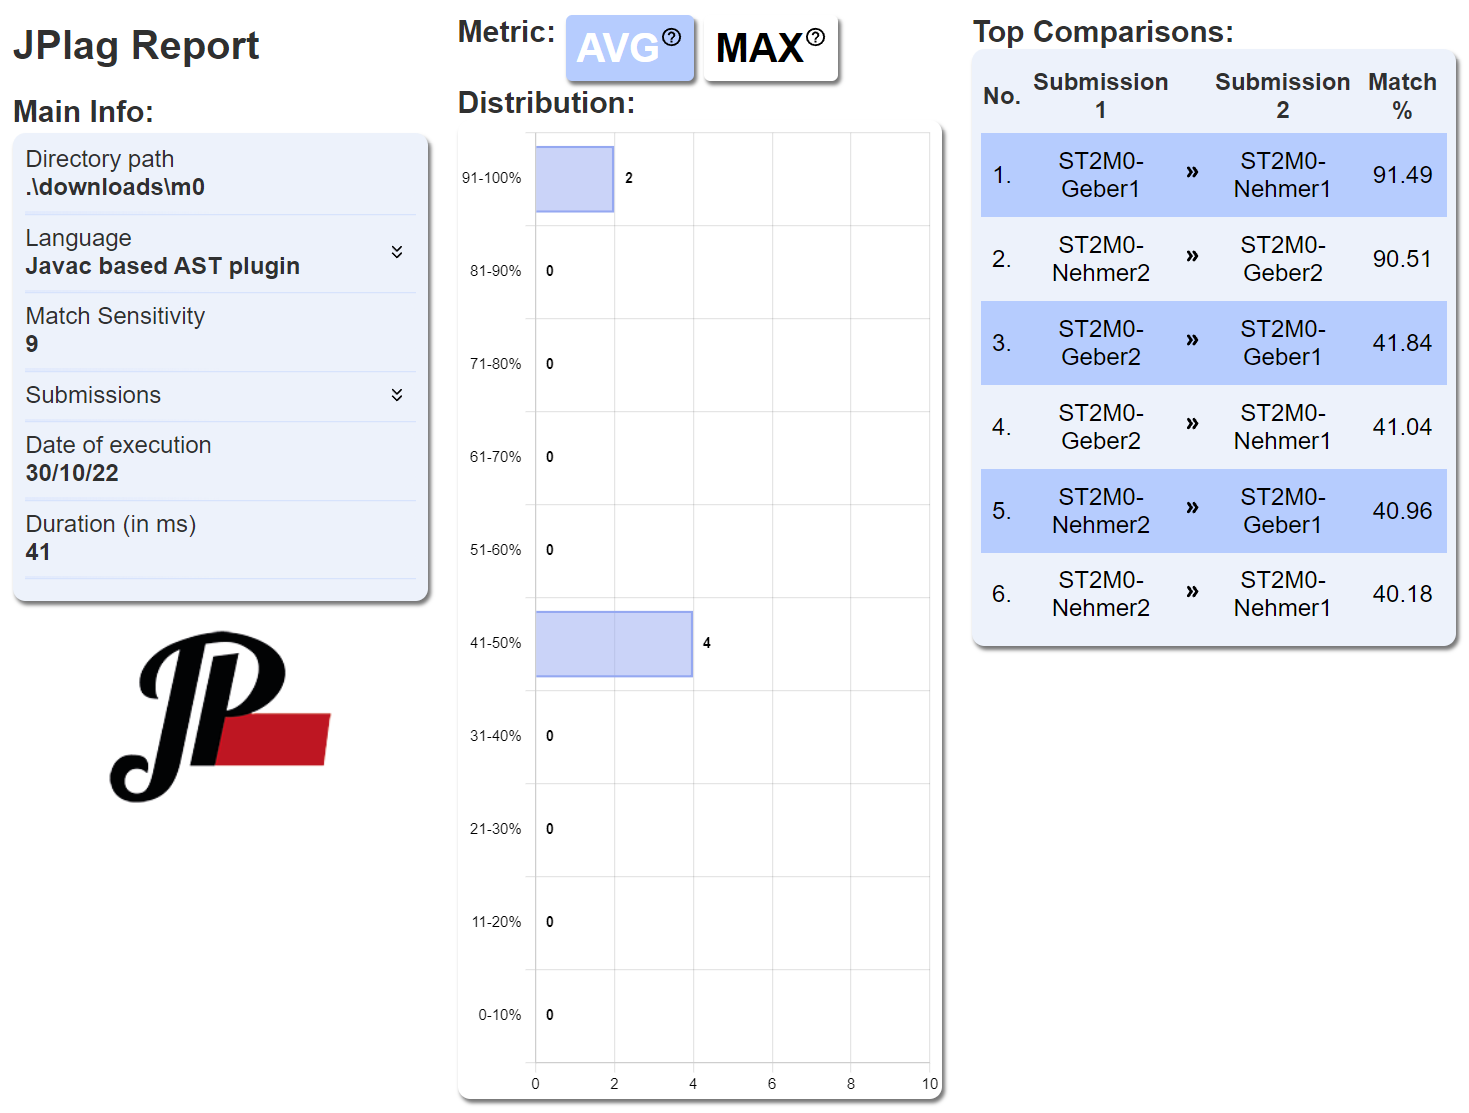
\includegraphics[scale=0.3]{figs/JPlag/JPlag_Overview.png}
	\caption{The JPlag overview showing the similarities of m0 code}
\end{figure}
When using JPlag to check the similarity of known plagiarized code it had similarity value for the plagiarized m0 code of 91.49\& and 90.51\% while the
none plagiarized code had similarity of around 40\%.
The results for m4 were somewhat less clear since they had a similarity value of 84.77\% and 76.2\%. Which should still lead to an investigation
of the submitted code.

\begin{table}[h]
	\centering
	\begin{tabular}{{|l|l|l|l|}}
		\hline
		Submission 1  & Submission 2  & Similarity  & Similarity with base code\\ \hline
		ST2M0-Geber1  & ST2M0-Nehmer1 & 91.49\%  & 88.11\% \\ \hline
		ST2M0-Nehmer2  & ST2M0-Geber2 & 90.51\%  & 86.11\% \\ \hline
		ST2M0-Geber2  & ST2M0-Geber1 & 41.84\%   & 16.34\% \\ \hline
		ST2M0-Geber2 & ST2M0-Nehmer1 & 41.04\%   & 16.21\% \\ \hline
		ST2M0-Nehmer2  & ST2M0-Geber1  & 40.96\% & 14.61\% \\ \hline
		ST2M0-Nehmer2  & ST2M0-Nehmer1 & 40.18\% & 14.56\% \\ \hline
	\end{tabular}
	\centering
	\caption{\label{tab:JPlagSimilarityTableM0}[Table of Milestone [0] showing the similarity between submissions]}
\end{table}

It should also be noted that no files were excluded and that there was no base code passed to JPlag, which explains the high similarity between unrelated
programs as all submissions for a milestone use the same base code. When excluding common base code then the results for m0 become significantly more clear
with the known plagiarism having a similarity value between 86 and 89 percent while the none plagiarized submissions have a value between 14 and 17 percent.

Looking at m4 with the base code excluded still shows a less clear image. With the known plagiarized have a similarity value which is lower by 9 to 7 percentage
points and with the none plagiarized submissions having a similarity value which lower by 18 to 16 percentage points. All of which are considerably smaller percentage
point drops then those observed in m0. It is not clear why exactly the similarity values of m4 are closer to each other in m4 and why the difference between them doesn't
grow that much when excluding the base code in comparison to m0.

\begin{table}[h]
	\centering
	\begin{tabular}{|l|l|l|l|}
		\hline
		Submission 1   & Submission 2  & Similarity  & Similarity with base code\\ \hline
		ST2M4-Nehmer2  & ST2M4-Geber   & 84.47\% & 77.97\% \\ \hline
		ST2M4-Nehmer2  & ST2M4-Nehmer1 & 77.48\% & 68.30\% \\ \hline
		ST2M4-Geber    & ST2M4-Nehmer1 & 76.20\% & 67.42\% \\ \hline
		ST2M4-Nehmer2  & ST2M4-NoPlag2 & 49.00\% & 32.70\% \\ \hline
		ST2M4-Geber    & ST2M4-NoPlag2 & 47.20\% & 30.97\% \\ \hline
		ST2M4-Nehmer1  & ST2M4-NoPlag2 & 46.16\% & 29.90\% \\ \hline
		ST2M4-Nehmer1  & ST2M4-NoPlag1 & 41.82\% & 25.33\% \\ \hline
		ST2M4-Nehmer2  & ST2M4-NoPlag1 & 40.55\% & 22.78\% \\ \hline
		ST2M4-Geber    & ST2M4-NoPlag1 & 39.99\% & 22.69\% \\ \hline
		ST2M4-NoPlag2  & ST2M4-NoPlag1 & 36.40\% & 20.15\% \\ \hline
	
	\end{tabular}
	\caption{\label{tab:JPlagSimilarityTableM4}[Table of Milestone [4] showing the similarity between submissions]}
\end{table}

%\subsubsection{Integration into an automated evaluation pipeline}

%JPlag probably show the most potential to be used in an automated pipeline as it not only provides a CLI but also a Java API, while also being able to be
%run locally\autocite{JPlagG} which means that there are no submission limits like in MOSS and that JPlag can be easily integrated into the existing pipeline.
%However, results are always saved as a Zip file and are view in a web application which can also be run locally. This poses a problem as???

%-How does the pipeline work, are files permanently saved or deleted after it finishes evaluation, can they be accessed

\subsection{Plaggie}

Plaggie was developed by Aleksi Ahtiainen, Sami Surakka and MIkko Rahikainen from the Helsinki University of Technology in 2006 in order to detect cheating in
Java exercises. It was written in Java 5 and can analyze Java 5 applications \autocite[3. Current list of features]{RMP}. With its most important
contribution at the time being the only open source plagiarism tool that could be run locally \autocite[p. 141]{PLAGGIE}.

\subsubsection{The Algorithm}

Plaggie uses CUP as a parser for which is a LALR parser that implements standard LALR(1) parser generation \autocite{CUP}. The algorithm to compare
the tokens extracted by CUP is GST which has been extended to exclude existing code but doesn't feature any other optimizations \autocite[4. Algorithm used]{RMP}.

Plaggie display the similarity of individual files and entire submissions. With the similarity of two files being the percentage of the matched tokens
in comparison to the total number of tokens in the file. The similarity of the submission A is the average of the best match of each file with the
submission similarity of submission B being the average of the corresponding similarity values in submission B \autocite*[4. Algorithm used]{RMP}. 

\subsubsection{Preliminary results}

We didn't manage to run Plaggie as it hasn't been updated since 2006 and we ran a newer version of Java which caused compilation error. However, based
on the fact that Plaggie only supports Java 1.5 and that JPlag has since been made open source Plaggie would not be our tool of choice since there are
more modern tools which are being actively maintained and have support for more modern programming languages.

There are some know successful and unsuccessful attacks identified by Plaggie's developers. With the unsuccessful attacks being:
\begin{itemize}
	\item "Changing the comments"
	\item "Changing the indentation"
	\item "Method and variable name changes"
	\item "Renaming the classes"
\end{itemize} \autocite*[Known successful attacks]{RMP}

and the unsuccessful attacks being:
\begin{itemize}
	\item "Moving inline code to separate methods and vice versa"
	\item "Inclusion of redundant program code"
	\item "Changing the order of if-else blocks and case-blocks"
\end{itemize}
\autocite[Known unsuccessful attacks]{RMP}

\newpage

\subsection{AC2}

"AC is a source code plagiarism detection tool. It aids instructors and graders to detect plagiarism within a group of assignments written in languages such as C, C++, Java, PHP, XML, Python, ECMAScript, Pascal or VHDL (plaintext works too, but is less precise). AC incorporates multiple similarity detection algorithms found in the scientific literature, and allows their results to be visualized graphically." \autocite{AC2} The first version of "AC was born in the Escuela Politécnica Superior of the Universidad Autónoma de Madrid to deter and detect source-code plagiarism in programming assignments". \autocite{AC2}

2016 AC version 2 was released. In the version 2.0 the developers switched to Maven and Antr4\footnote{\label{footnoteAntlr}"In computer-based language recognition, ANTLR (pronounced antler), or ANother Tool for Language Recognition, is a parser generator that uses LL(*) for parsing. ANTLR is the successor to the Purdue Compiler Construction Tool Set (PCCTS), first developed in 1989, and is under active development."\autocite{enwiki:1115716413}}. The developers of AC also moved their git repository to GitHub an internet hosting service for software development and version control.

AC2 lists some advantages over the other plagiarism detection tools on their GitHub page. In this regard, it is

\begin{itemize}
	\item "local, and does not require sending data to remote servers (not the case of Moss)local, and does not require sending data to remote servers (not the case of Moss)"
	\item "robust, using Normalized Compression Distance as its main measure-of-similarity, but with the possibility of integrating other, additional measures to gain better pictures of what is going on (JPlag, Moss and Plaggie have hard-coded analyses, mostly based on sub-string matching after tokenization)."
	\item "heavy on information visualization. AC will not provide "percentage of copy"; instead, it will create graphical representations of the degree of similarity between student submissions within a group, so instructors can build their own explanations regarding what really happened (see here and here for papers on AC's visualizations)."
\end{itemize}\autocite{AC2}

\subsubsection{AC2 comparison algorithm}
\label{sec:AC2ComparisonAlgorithm}

In order for the AC algorithm to check files for equality, it allows adding folders or zip-files into it. Two filters can be applied to these files. The first filter selects the submissions that will be examined, and the second filter is determining which files are compared to each other. 

For example student s1 has in his subfolder 'a.c' and student s2 has in his folder 'aa.c'. So the first filter should determine that each submission starts with the letter 's'. The second filter would look for files that ended with the string '.c'.

When all submission and files are correctly grouped together the analysis part can start. "The default analysis (Zip NCD), uses \hyperref[sec:NCD]{normalized compression distance (NCD)} to detect redundancy (= similarity) between submissions. If AC2 knows the programming language of its source files, they will be tokenized prior to comparison. This will allow AC2 to ignore comments, whitespace and exact identifiers, so that simply renaming variables or altering formatting will not affect similarity calculations." \autocite{AC2wiki} 

\paragraph{NCD (normalized compression distance)}
\label{sec:NCD}

\textcolor{red}{Todo: NCD beschreiben und sagen wie es in AC2 verwendet wird.}

\paragraph{Tokenization}

If AC2 can recognize the programming language it will use a lexer and a parser to tokenize the text file. "AC2 uses Antlr4\footref{footnoteAntlr} grammars to generate lexers (= tokenizers) and parsers for languages." \autocite{AC2wiki} Therefore it is relatively easy to add support for a new programming language.

\subsubsection{Preliminary results}

In order to present the advantages of AC2, several projects were compared using the AC2 algorithm. As explained in section~\ref{sec:AC2ComparisonAlgorithm} \nameref{sec:AC2ComparisonAlgorithm}, the filters were used to select and group the submissions. After passing the project files, the algorithm analyzes them and creates an output window. The output that AC2 generates is mainly visual based. So Ac "will create graphical representations of the degree of similarity between student submissions within a group". \autocite{AC2}. See figure~\ref{fig:AC2R1} and figure~\ref{fig:AC2R2}.

\begin{figure}[h]
	\centering
	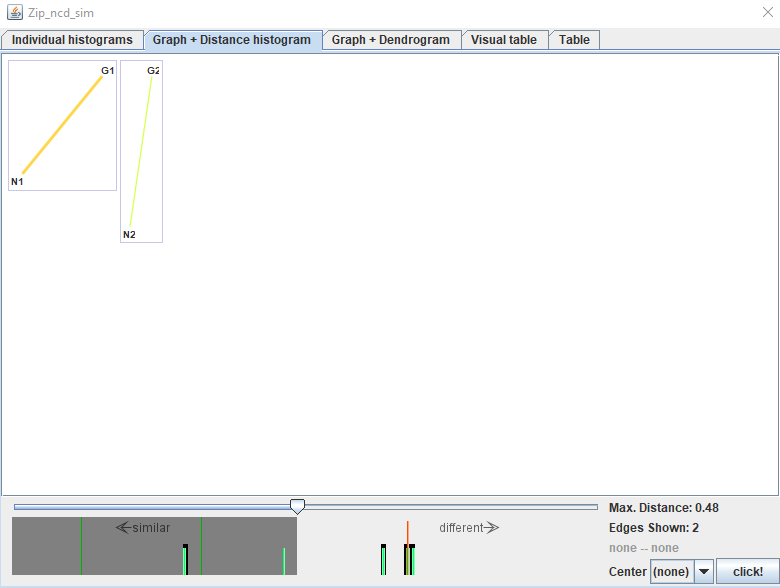
\includegraphics[height=0.2\textheight]{figs/AC2/M0_1.png}
	\caption{The graphical output of AC2 from milestone [0]}
	\label{fig:AC2R1}
\end{figure}
Figure~\ref{fig:AC2R1} shows milestone 0 and how the different projects have copied from each other. This suggests that project N1 has maybe copied its code form G2 and N2 from G2.

\begin{figure}[h]
	\centering
		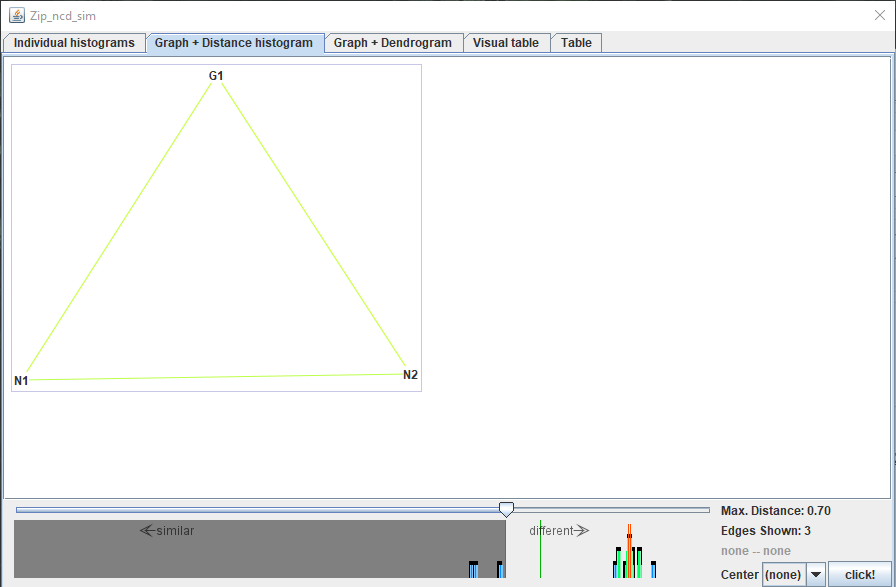
\includegraphics[height=0.2\textheight]{figs/AC2/M4_1.png}
		\caption{The graphical output of AC2 from milestone [4]}
		\label{fig:AC2R2}
\end{figure}

Figure~\ref{fig:AC2R2} illustrates that G1, N1 and N2 have probably copied from each other, since a correlation exists between the 3 projects. This again illustrates the advantage of AC2 over the other plagiarism detection programs, since it is easier to detect multiple correlations between projects.

\begin{table}[h]
	\begin{minipage}{.5\textwidth}
		\centering
		\scalebox{0.9}{
			\begin{tabular}{{|l|l|l|}}
				\hline
				One           & The other     & Distance \\ \hline
				ST2M0-Geber1  & ST2M0-Nehmer1 & 0.2926   \\ \hline
				ST2M0-Geber2  & ST2M0-Nehmer2 & 0.4609   \\ \hline
				ST2M0-Geber1  & ST2M0-Nehmer2 & 0.6302   \\ \hline
				ST2M0-Nehmer2 & ST2M0-Nehmer1 & 0.6705   \\ \hline
				ST2M0-Geber2  & ST2M0-Geber1  & 0.6718   \\ \hline
				ST2M0-Geber2  & ST2M0-Nehmer1 & 0.6811   \\ \hline
			\end{tabular}
		}
		\caption{\label{tab:AC2DistanceTableM0}[Table of Milestone [0] distance between projects]}
	\end{minipage}%
	\begin{minipage}{.5\textwidth}
		\centering
		\scalebox{0.9}{
			\begin{tabular}{|l|l|l|}
				\hline
				One           & The other     & Distance \\ \hline
				ST2M4-Geber1  & ST2M4-Nehmer2 & 0.6538   \\ \hline
				ST2M4-Geber1  & ST2M4-Nehmer1 & 0.6603   \\ \hline
				ST2M4-Nehmer2 & ST2M4-Nehmer1 & 0.6957   \\ \hline
				ST2M4-NoPlag2  & ST2M4-Nehmer1 & 0.6809   \\ \hline
				ST2M4-Geber1  & ST2M4-NoPlag1  & 0.8647   \\ \hline
				ST2M4-NoPlag1  & ST2M4-Nehmer1 & 0.8657   \\ \hline
				ST2M4-NoPlag2  & ST2M4-NoPlag1  & 0.8772   \\ \hline
				ST2M4-NoPlag1  & ST2M4-Nehmer2 & 0.8792   \\ \hline
				ST2M4-NoPlag2  & ST2M4-Nehmer2 & 0.8809   \\ \hline
				ST2M4-NoPlag2  & ST2M4-Geber1  & 0.8823   \\ \hline
			
			\end{tabular}
		}
		\caption{\label{tab:AC2DistanceTableM4}[Table of Milestone [4] distance between projects]}
	\end{minipage}
\end{table}

Table~\ref{tab:AC2DistanceTableM0} and table~\ref{tab:AC2DistanceTableM4} show how far apart the individual projects are. This distinguishes AC2 from other plagiarism detection programs, as they often reflect the similarity in percent to the user.

\newpage


\section{Conclusion}

\newpage

\printbibliography[
	heading=bibintoc,
	title={References}
]

\appendix

\end{document}